\section{Results}
\label{sec:usage:results}

The specific queries given by the VS and the corresponding oracle labels 
(the oracle, in this case, is the author of this work) may be seen in 
Figures~\ref{fig:usage:interesting} and \ref{fig:usage:notinteresting}. Recall 
that the active learner in stage 1 was given a budget of 15 queries. The 
queried plots are not labeled during stage 1 in order to prevent potential bias 
from clouding the oracle's responses. After stage 2, the user may plot and view 
the corresponding variable names should he/she wish to do so.

\newpage 
\begin{figure}[htb]
	\begin{center}
		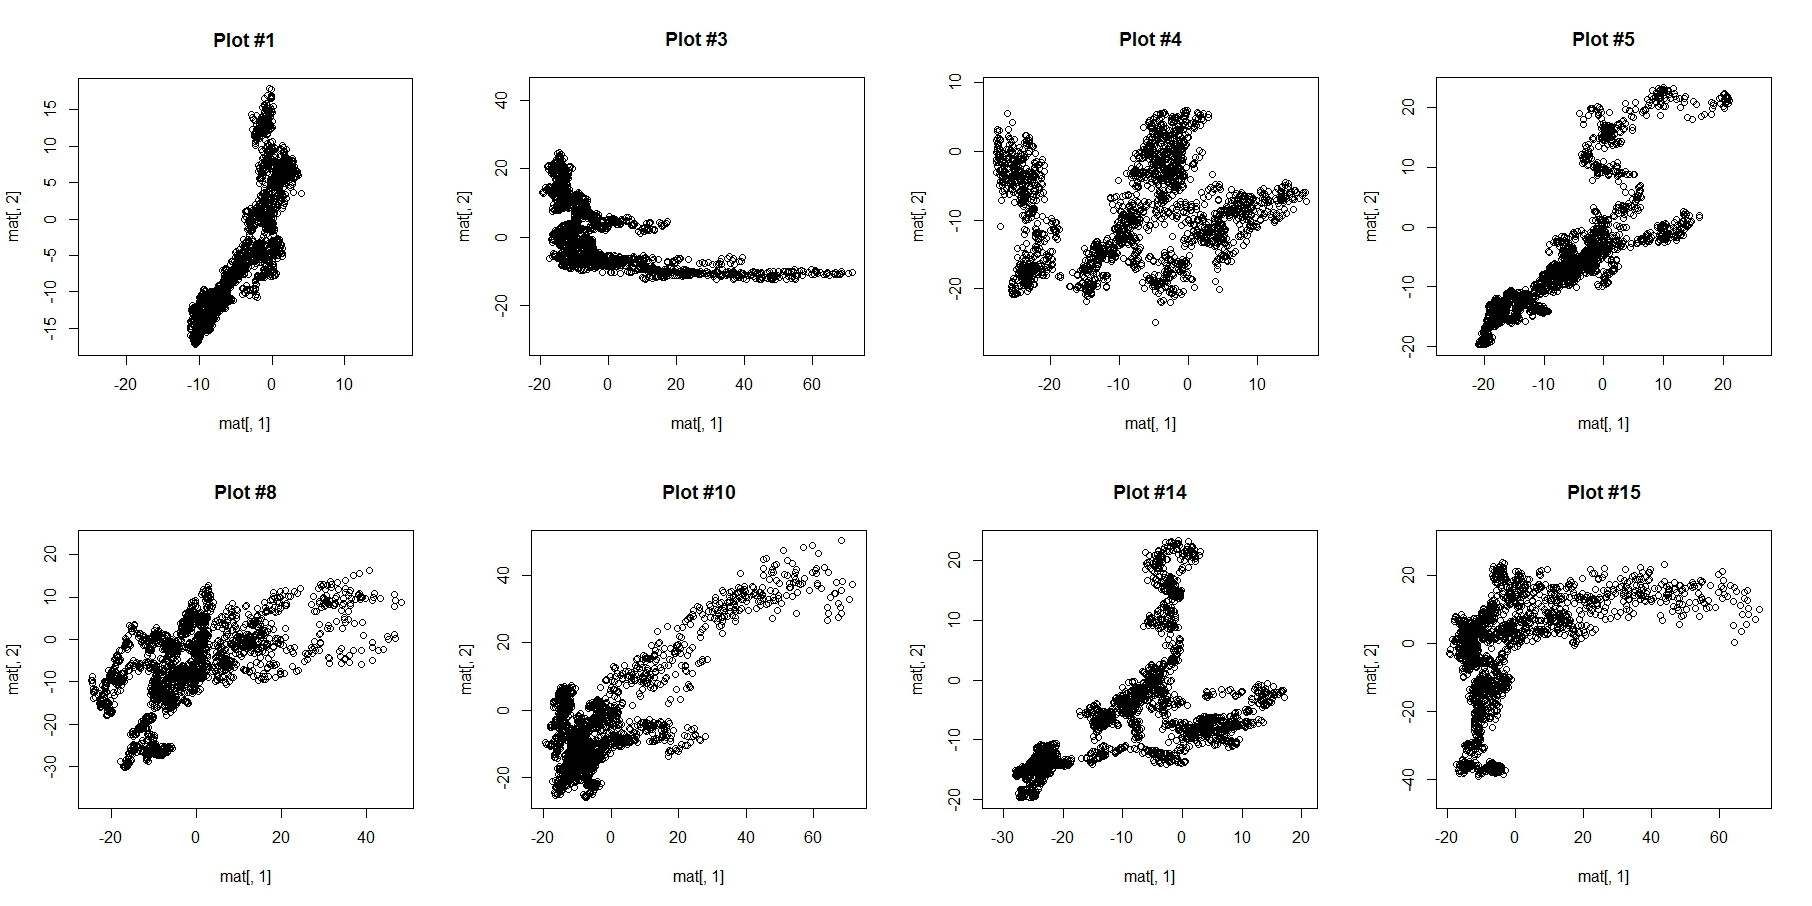
\includegraphics[width=1\linewidth]{ch-usage/figures/y_all}
		\caption[VS queries which were labeled ``visually correlated''.]{VS 
		queries which were labeled ``visually correlated''.}
		\label{fig:usage:interesting}
	\end{center}
\end{figure}

\begin{figure}[H]
	\begin{center}
		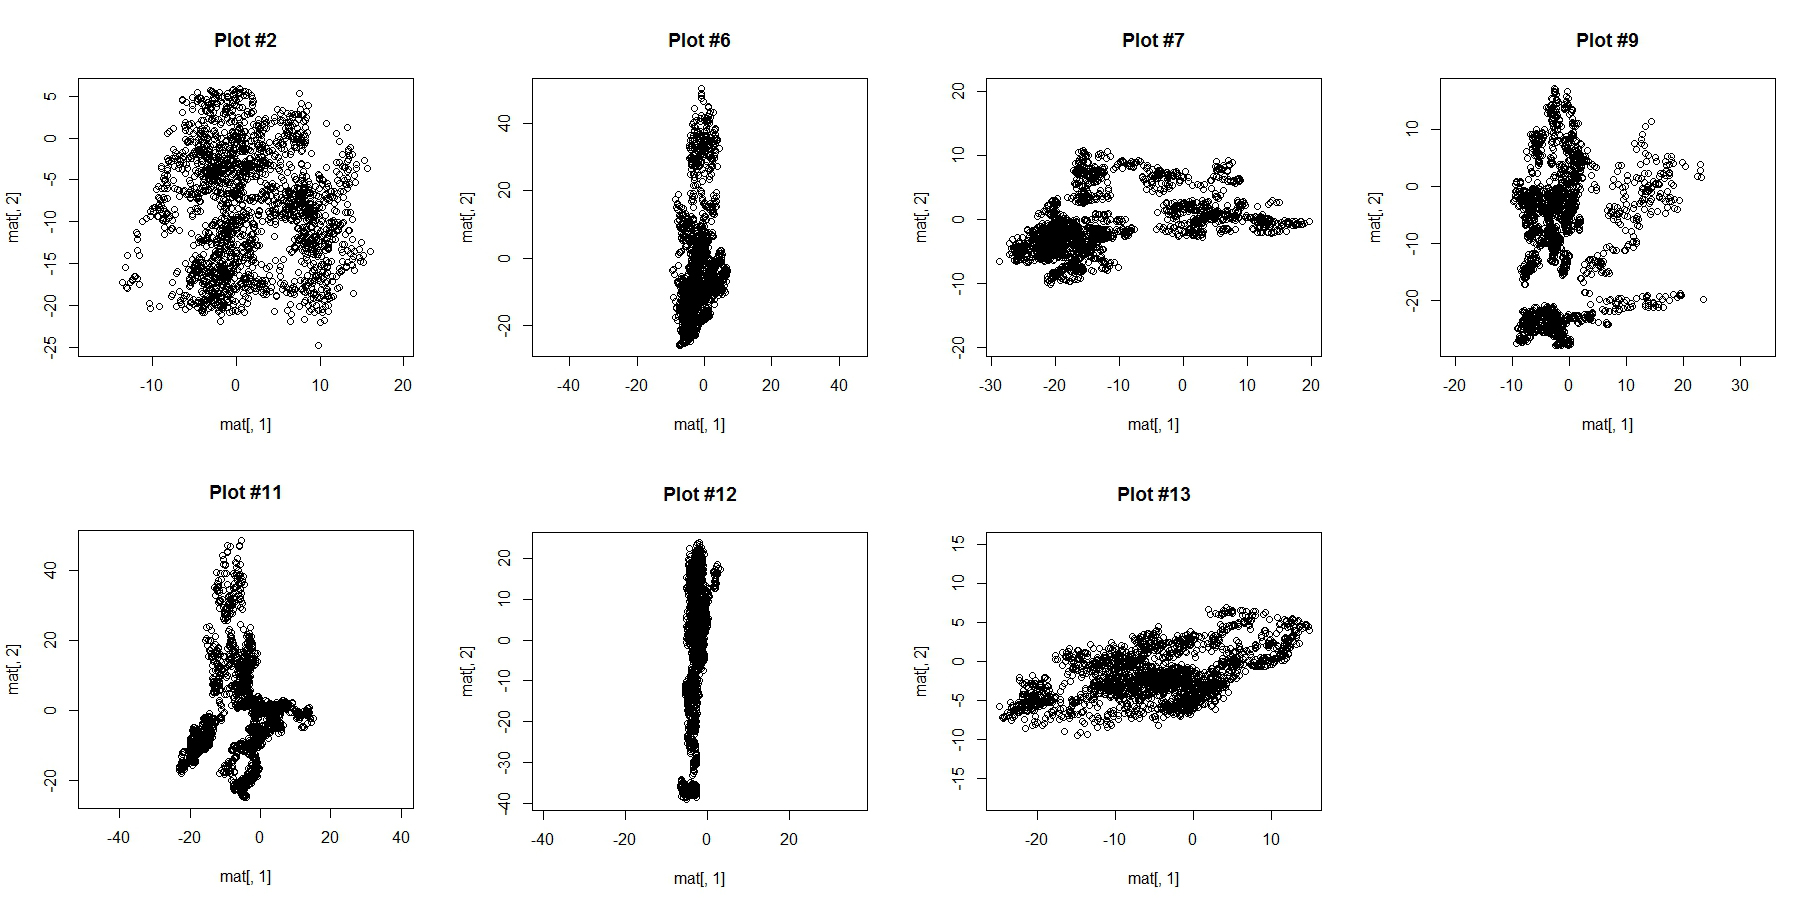
\includegraphics[width=1\linewidth]{ch-usage/figures/n_all}
		\caption[VS queries which were labeled ``not visually correlated''.]{VS 
		queries which were labeled ``not visually correlated''.}
		\label{fig:usage:notinteresting}
	\end{center}
\end{figure}

It is also interesting to examine the heat maps (which are normalized) that 
correspond to the 15 queries; these heat maps may be found 
in Figure~\ref{fig:usage:heatmaps}, which also contains a list of associated 
criterion. A quick glance at the heat maps reveal that 
the middle criteria are all zero. It actually turns out that these criteria 
are associated with various Pearson correlation tests. 
The zero-value heat map entries indicate that the associated $p$-values are all 
extremely low (the correlation is significantly different from zero). In 
particular, this indicates that the criterion 9, 10, 11, 12, 13, and 14 are 
all significant. Consider the actual variable pairs associated with these 
criteria. The first row corresponds to the first queried plot which received a 
label of ``not visually interesting'' (It is the top left plot depicted in 
Figure~\ref{fig:usage:notinteresting}). Specifically, the pair has a Pearson 
correlation coefficient of -0.069 and $p$-value of 0.001728. The Pearson 
correlation coefficient is actually rather close to 0 
(uncorrelated) despite the $p$-value suggesting otherwise. When looking at the 
metric numerically as the heat map does, the natural response would be to draw 
an edge as in the $p$-value heuristic given in 
Section~\ref{sec:intro:correlation}. 
However, visually examining the pair's scatter plot (and even just looking at 
the correlation coefficient without the $p$-value) makes it clear that the pair 
is uncorrelated. How did this happen? Because there are 2050 observations of 
each stock, the variance, and subsequently the $p$-value, is low. 
If the correlation graph was constructed solely based on 
the Pearson correlation coefficient $p$-value without consideration of other 
factors, the result would have been less than ideal. This is another scenario 
that demonstrates the usefulness of the VS.

\begin{figure}[H]
	\begin{center}
		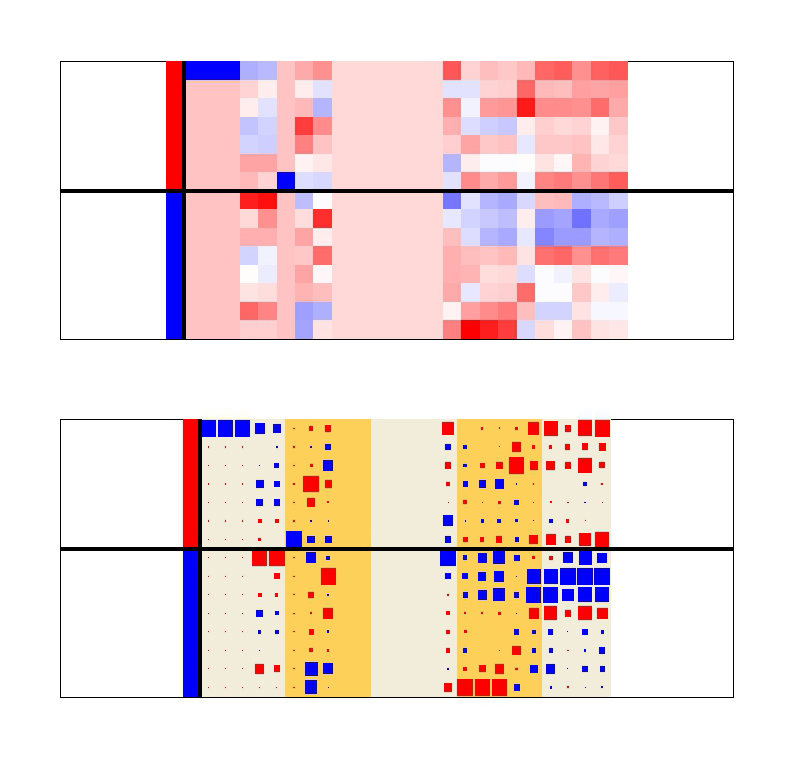
\includegraphics[width=0.8\linewidth]
		{ch-usage/figures/heatmaps}
		\caption[Normalized heat maps of VS queries and user-specified labels.] 
		{\textit{Top:} Standard heat map of the queries and given labels 
		(normalized). 
		\textit{Bottom:} Revised heat map (the association navigator) as 
		proposed by Buja \textit{et al.}~\cite{buja2016} (also normalized). 
		Each row corresponds to a pairwise scatter plot queried by the VS in 
		stage 1. Each scatter plot is ordered by 
		the oracle's responses; red indicates ``not visually correlated'' 
		and blue indicates ``visually correlated'' (as dictated by the 
		oracle). Each column 
		corresponds to a different criterion of the associated pairwise 
		scatterplot (see Section~\ref{sec:visualizer:scatterplot}). Ordered 
		criterion list (left to right, up to down): 
		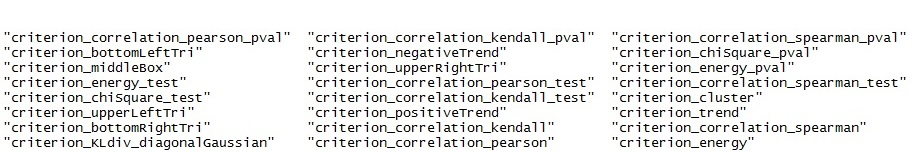
\includegraphics[width=1\linewidth]{ch-usage/figures/criterionlist}}
		\label{fig:usage:heatmaps}
	\end{center}
\end{figure}

Figure~\ref{fig:usage:hist} is a predicted probability histogram. The 
probability of being ``visually interesting'' or not is computed for 100 random 
pairwise scatter plots. Each probability is computed using the final 
classifier output from stages 1 and 2 of the VS. Most of the pairs fall within 
two bins (low and high probability). This can be observed as the two upper and 
lower hills in the histogram, indicating that the final classifier 
determined by the VS is quite confident in its labeling of most of the scatter 
plots.

\begin{figure}[htb]
	\begin{center}
		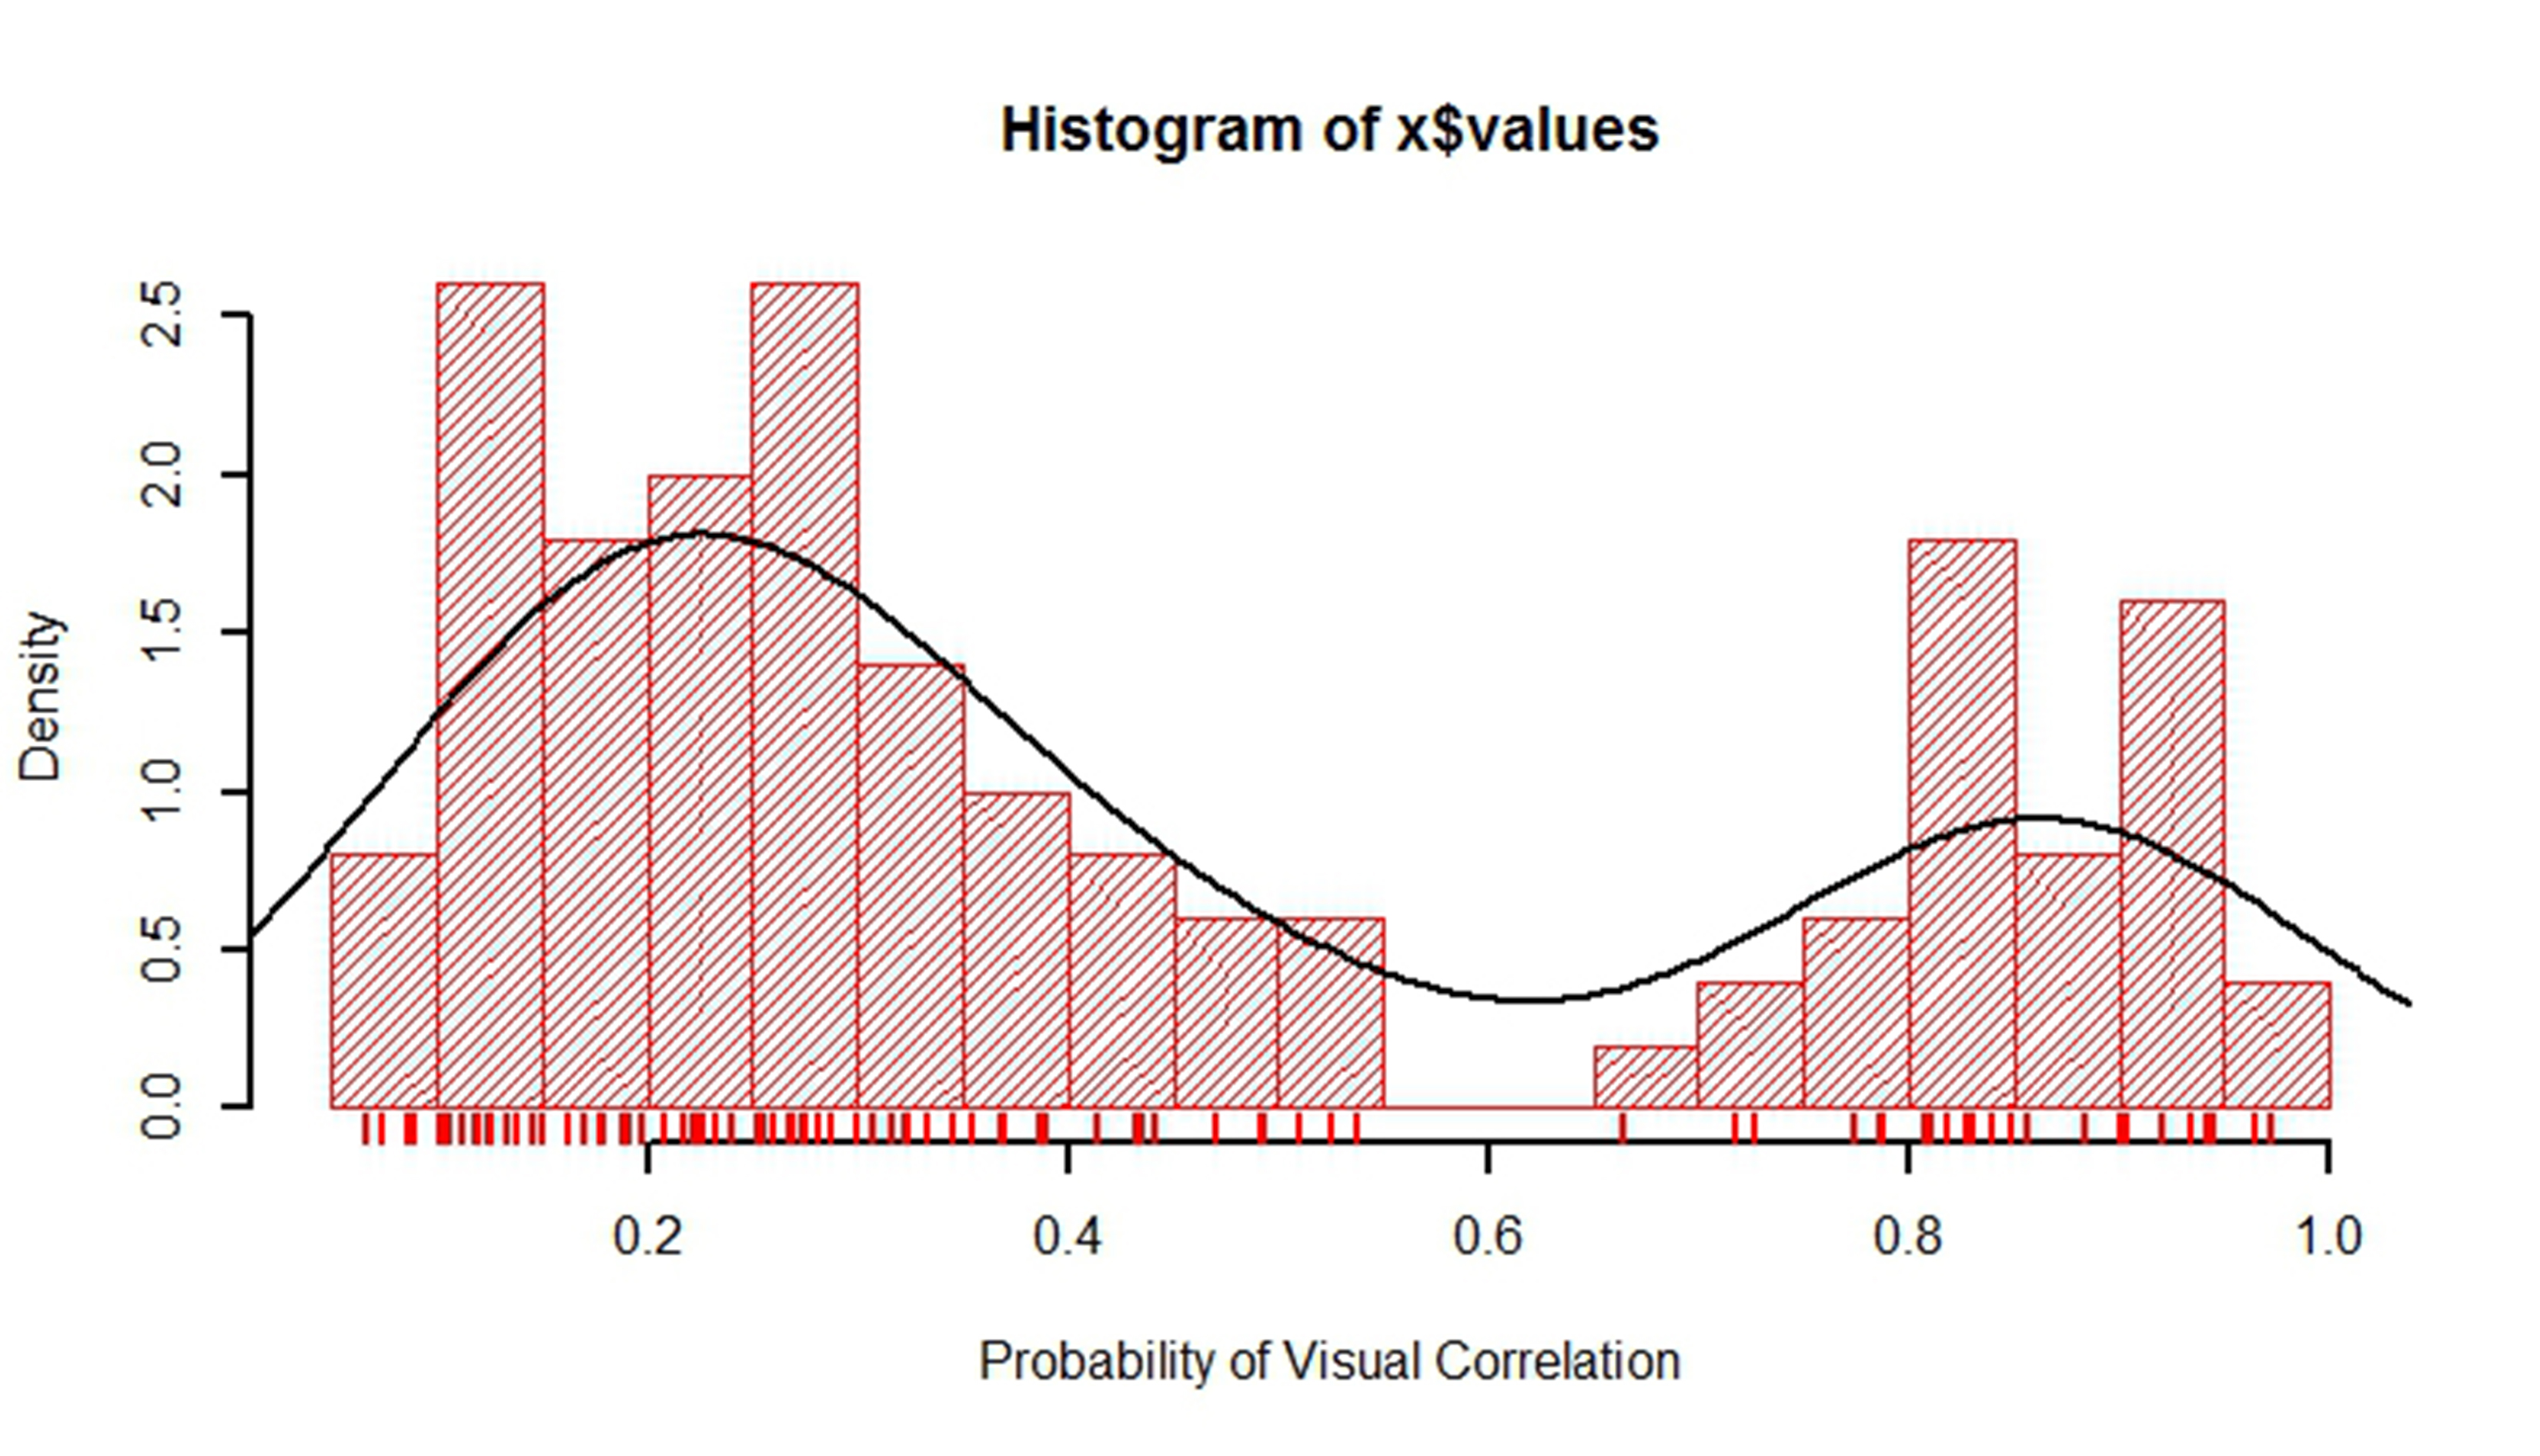
\includegraphics[width=1\linewidth]
		{ch-usage/figures/predicted_probability_histogram}
		\caption[Histogram of predicted probabilities.]{The histogram shows the 
		predicted probabilities for 100 pairwise scatter plots. The 
		probability corresponds to the probability of a plot being 
		``visually correlated'' or ``not visually correlated''.}
		\label{fig:usage:hist}
	\end{center}
\end{figure}

\begin{figure}[htb]
	\begin{center}
		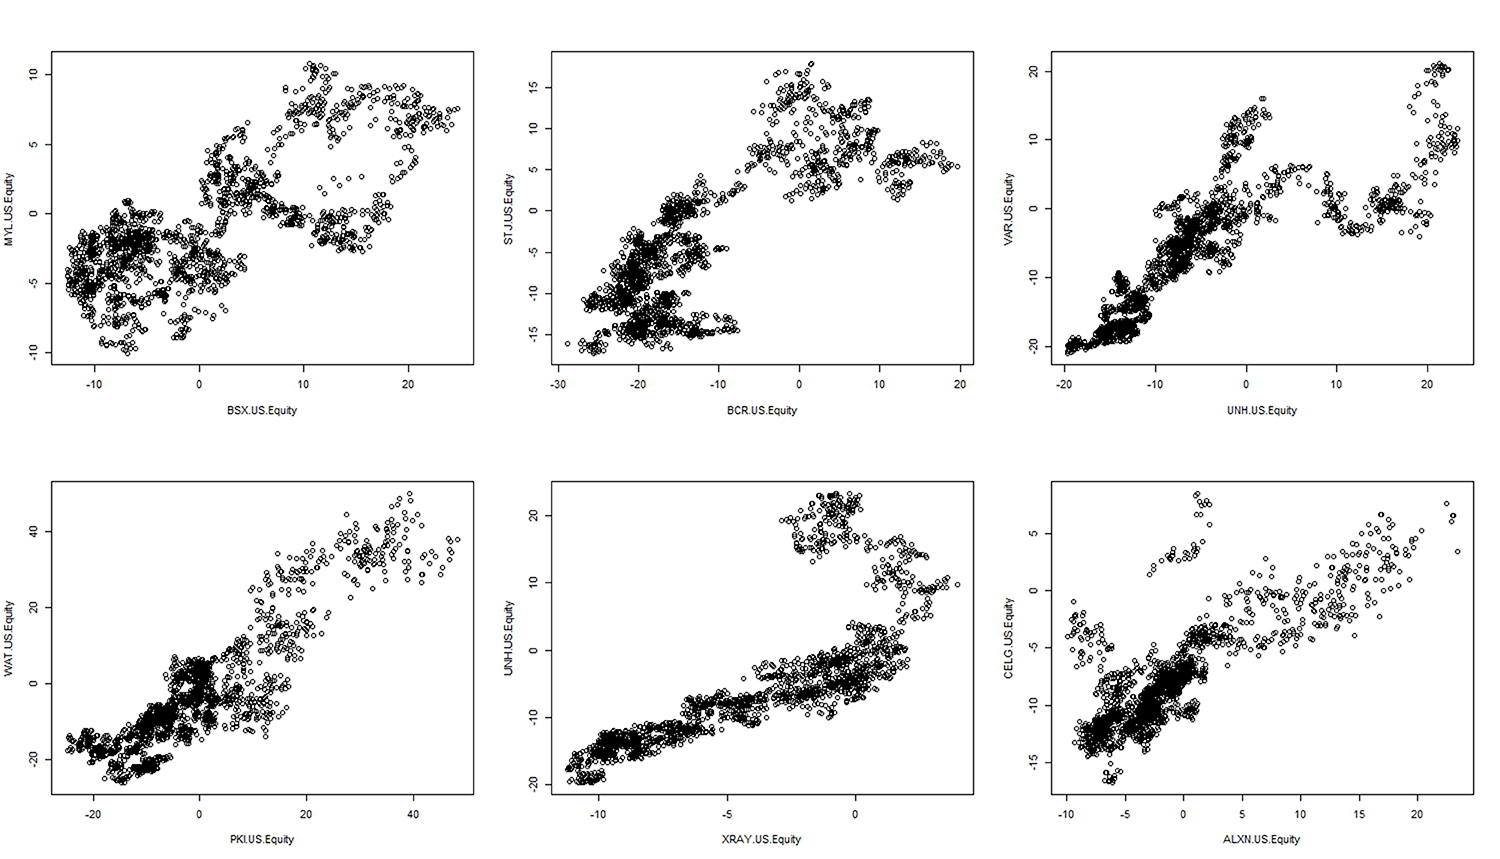
\includegraphics[width=1\linewidth]
		{ch-usage/figures/topinterestingplots}
		\caption[Top six most ``visually correlated'' pairwise scatter plots	
		selected by the VS.]{Top six most ``visually correlated'' pairwise 
		scatter plots selected by the VS.}
		\label{fig:usage:interestingplots}
	\end{center}
\end{figure}

\newpage
Figure~\ref{fig:usage:interestingplots} contains the most interesting plots 
selected by the VS in the automatic plot generation output of the VS. 
Interestingly, none of the variables (stocks) which are involved in these plots 
ever show up twice. Most of these plots exhibit a strong positive trend.
The final resulting visual correlation graph is shown in 
Figure~\ref{fig:usage:visg}. Interestingly, only stock 39 (which corresponds to 
ticker TMO) is in its own cluster; in fact, its degree is zero! This indicates 
that TMO is one of the best stocks to select because it is ``visually not 
correlated'' and, by proxy, independent of all other stocks.

\begin{figure}[H]
	\begin{center}
		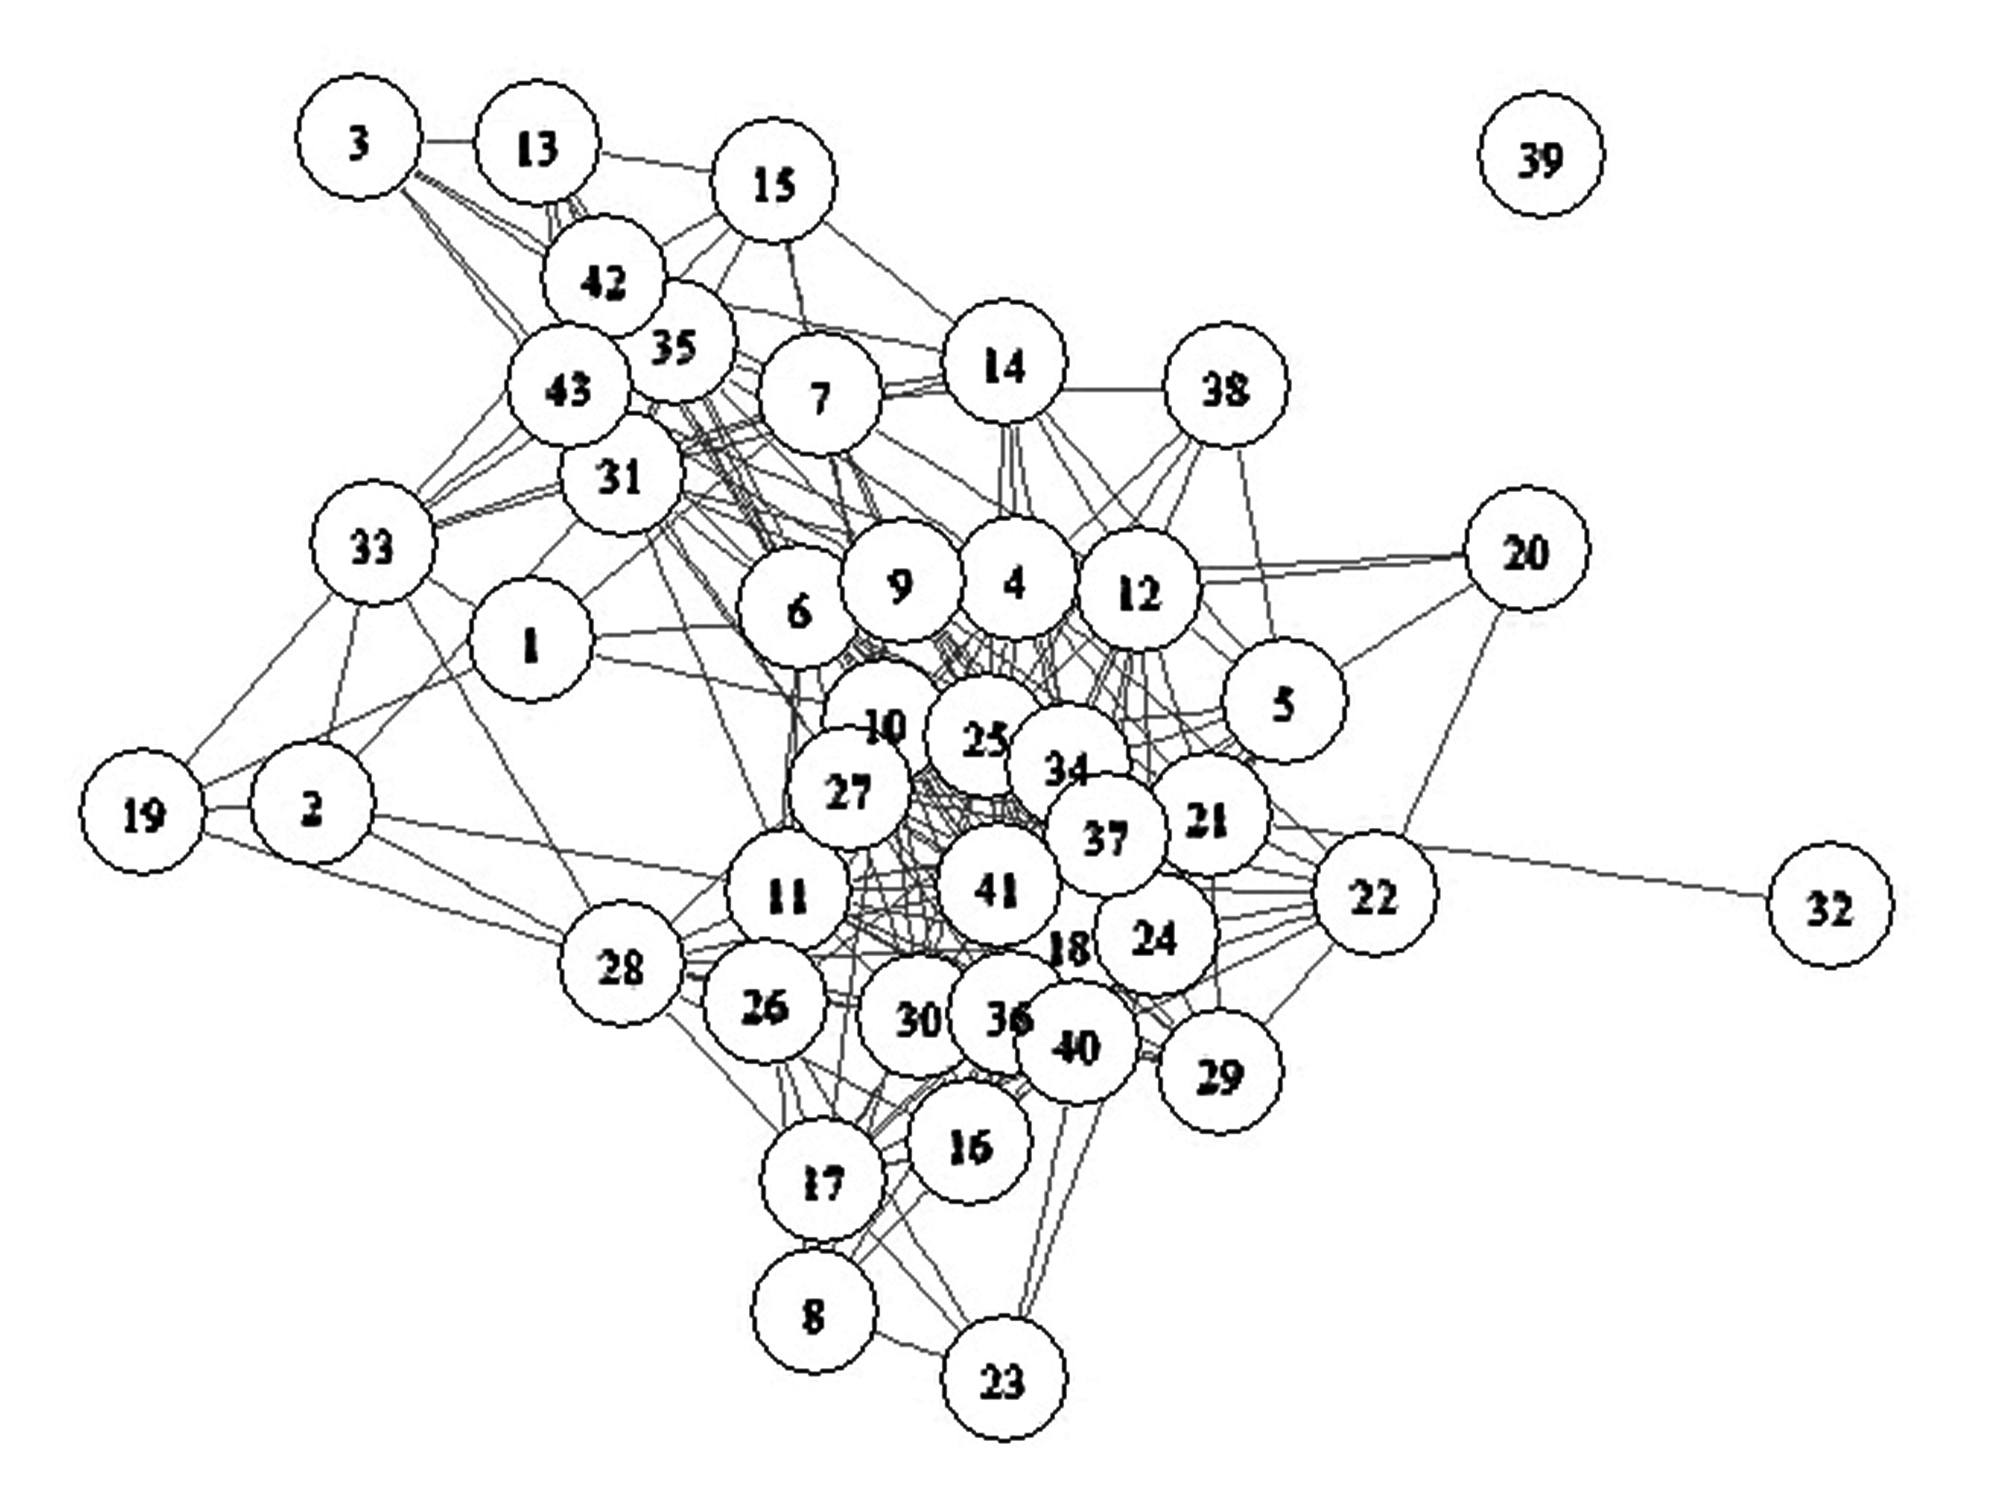
\includegraphics[width=0.75\linewidth]
		{ch-usage/figures/visgraph}
		\caption[Visual correlation graph output from the visualization 
		system.]{Visual correlation
		graph output from the visualization system.}
		\label{fig:usage:visg}
	\end{center}
\end{figure}

The graph comparison procedure determined that the \textbf{distance correlation 
graph} is closest to the visual correlation graph. 
The computed graph differences may be found in Table~\ref{tab:usage:graphdiff}.
The resulting portfolios selected by the procedure in 
Section~\ref{sec:usage:stockselection} for each numerical correlation graph are 
summarized in Table~\ref{tab:usage:returns}. Only the Pearson's correlation 
graph and distance correlation graph include TMO, the most ``visually not 
correlated'' stock, in their portfolios. 

Finally, the the ``buy and hold'' performance (yearly returns) and cumulative 
sum of returns are plotted for the S\&P 500 (the control) and
all portfolios $P^i$ for $i \in \{1,...,4\}$ may be found in 
Figure~\ref{fig:usage:returns}. Each portfolio $P^i$ was created 
from its corresponding numerical correlation graph $\hat{G}^{i,\text{num}}$ and 
includes $P^*$, which is created from $\hat{G}^* = \hat{G}^{4,\text{num}}$ 
(which corresponds to the distance correlation graph). The associated 
data may be found in Table~\ref{tab:usage:returns}. Note 
that the returns for 2006 and 2014 are low because the data begins 
on 3/14/2006 and ends on 5/13/2004; as such, the returns for 2006 and 2014 do 
not reflect a full year's worth of data. Our focus is mostly diverted to the 
full years in between and especially the portfolio performance during the 
financial crisis. 

The portfolio $P^*$, constructed from the numerical distance correlation graph 
$\hat{G}^*$ that is most similar to the visual correlation graph $\hat{G}$, 
performs the strongest by far. $P^*$ consistently posts the highest returns 
year after year. Though it doesn't seem to strongly outperform on a yearly 
basis, the differences really add up as can be seen in cumulative sum of yearly 
returns. Further 
consider the financial crisis; $P^*$ has the least negative returns of 2008. 
This indicates that the visual graph is capturing the independence and 
dependence among various stocks properly, which translates into the selection 
of $\hat{G}^*$ and, subsequently, $P^*$, a portfolio that is well balanced and 
captures the spirit of the ``buy and hold'' model described in 
Section~\ref{sec:intro:finance}.
Although the Pearson's correlation portfolio also included TMO, it 
performed rather average; it seems that linearity was not enough to 
capture the relationships among the other stocks.
As noted earlier in Section~\ref{sec:usage:stockselection}, the proposed stock 
selection strategy is simple, but every selected portfolio has outperformed the 
S\&P 500, suggesting that an even more sophisticated selection procedure would 
yield even more fruitful returns.

\subsubsection{Extensions}

It should also be noted that, while a rebalancing method performs better in 
practice~\cite{liuh2016}, the ``buy and hold'' strategy is better-suited for 
observing portfolio performances over time with less external influences, 
providing a more concrete basis of comparison for $\hat{G}^*$. 
However, the procedure described in Section~\ref{sec:usage:newanalysis}
can certainly be repeated yearly (once a year's worth of new data has been 
collected) to determine the direction in which to 
rebalance the portfolio. Furthermore, the weights of the stocks in the 
portfolio can certainly be optimized; currently, each stock holds equal 
weight within its portfolio. All of these ideas are 
potential extensions that may improve upon portfolio management techniques that 
this application does not utilize.

%$P^{\text{vis}}$ catches up after a mediocre beginning, and there are other 
%interesting things to note about its performance that makes it difficult to 
%definitively say which portfolio is ``better''. Consider the financial crisis; 
%while the positive returns and recovery of $P^{\text{vis}}$ are muted, it has 
%the most significant least negative returns of 2008. This is an indication
%that the visual graph is capturing precisely what we wish for it to capture 
%(independence and dependence among various stocks), which is translating into 
%a portfolio that is well balanced and captures the spirit of the ``buy and 
%hold'' model described in Section~\ref{sec:intro:finance}. The persistence in 
%holding the portfolio ends up paying off returns rapid increase until the 
%portfolio is the top performer in 2011 and beyond.

\begin{landscape}
	\tablespacing
	\begin{longtable}{p{0.1\linewidth}p{0.15\linewidth}p{0.13\linewidth}
			p{0.13\linewidth}p{0.13\linewidth}p{0.13\linewidth} }
		
		% First page heading
		\caption[Computed differences between visual and numerical correlation 
		graphs.]{Computed differences between visual and numerical correlation 
		graphs. See Section~\ref{sec:gc:methods} for details on each graph 
		summarization metric.} 
		\label{tab:usage:graphdiff}\\
		\toprule
		\textbf{Graph Type} & \textbf{Centrality \newline (degree)} & 
		\textbf{Centrality \newline (closeness)} & 
		\textbf{Centrality \newline (betweenness)} & 
		\textbf{Assortativity} & \textbf{Distance \newline matrix} \\
		\midrule
		\endfirsthead
		
		% Last page footer
		\bottomrule
		\endlastfoot

		Pearson's & 0.0034 & 0.0119 & 0.0032 & 0.061 & 0.0313\\
		
		Spearman's & 0.0052 & 0.0079 & 0.0032 & 0.0773 & 0.029\\
		
		Kendall's & 0.0002 & 0.019 & 0.0024 & 0.0559 & 0.0253\\
		
		Distance & 0.0018 & 0.0276 & 0.0012 & 0.0465 & 0.0206\\
		
		\midrule
		
		& \textbf{Community\newline (random walk)} & 
		\textbf{Community \newline (infomap)} & 
		\textbf{Community \newline (betweenness)} & 
		\textbf{Edge\newline connectivity} & 
		\textbf{Edge density \newline histogram} \\
		 	
		\midrule
		
		Pearson's & 0.7602 & 0.5039 & 0.6488 & 1 & 0.6014\\
		
		Spearman's & 0.8478 & 0.5039 & 0.6948 & 1 & 0.5625\\
		
		Kendall's & 1 & 0.5039 & 0.7284 & 1 & 0.4413\\
		
		Distance & 0.253 & 0.5039 & 0.5437 & 1 & 0.2455\\
		
	\end{longtable}
	\bodyspacing
\end{landscape}





\begin{figure}[htb]
	\begin{center}
		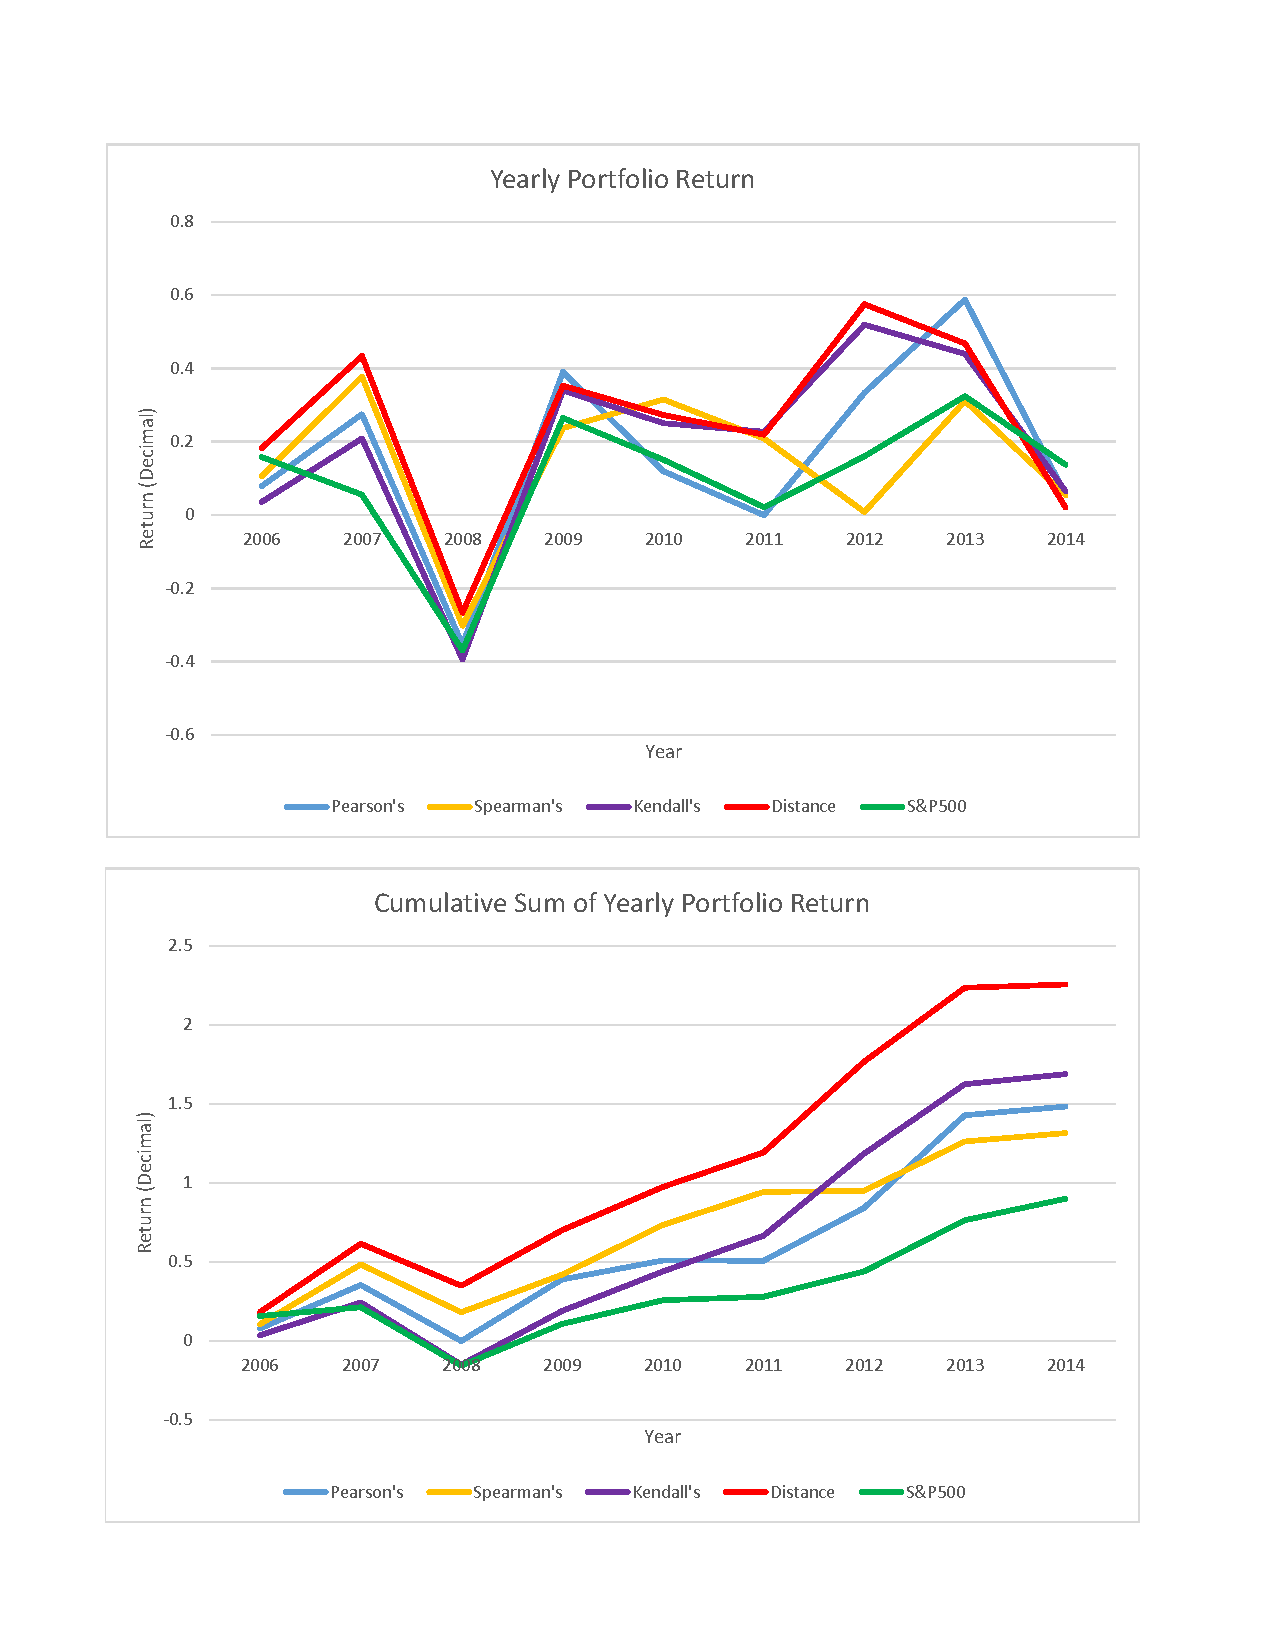
\includegraphics[width=1\linewidth]
		{ch-usage/figures/Results_YearlyReturns.pdf}
		\caption[Yearly and cumulative performance of the selected portfolios 
		and the S\&P 500.]{Yearly and cumulative performance of the selected 
		portfolios and the S\&P 500. Note that the ``yearly'' returns for 2006 
		and 2014 are low because the data begins on 3/14/2006 and ends on 
		5/13/2004; as such, those returns do not reflect a full year of data. 
		The associated data may be found in Table~\ref{tab:usage:returns}.}
		\label{fig:usage:returns}
	\end{center}
\end{figure}




\begin{landscape}
\tablespacing
\begin{longtable}{p{0.15\linewidth}p{0.15\linewidth}p{0.05\linewidth}
p{0.05\linewidth}p{0.05\linewidth}p{0.05\linewidth} 
p{0.05\linewidth}p{0.05\linewidth}p{0.05\linewidth} 
p{0.05\linewidth}p{0.05\linewidth}p{0.05\linewidth} 
p{0.05\linewidth}}
	
	% First page heading
	\caption[Yearly returns of the portfolios selected from the numerical 
	correlation graphs.]{Yearly returns (in decimal) of the portfolios selected 
	from the numerical correlation graphs.} 
	\label{tab:usage:returns}\\
	\toprule
	\textbf{Graph Type} & \textbf{Portfolio} & \textbf{2006} 
	& \textbf{2007} & \textbf{2008} & \textbf{2009} & 
	\textbf{2010} & \textbf{2011} & \textbf{2012} & 
	\textbf{2013} & \textbf{2014} \\
	\midrule
	\endfirsthead
	
	% Future page heading
	\caption[]{(continued)}\\
	\toprule
	\textbf{Graph Type} & \textbf{Portfolio} & \textbf{2006} 
	& \textbf{2007} & \textbf{2008} & \textbf{2009} & 
	\textbf{2010} & \textbf{2011} & \textbf{2012} & 
	\textbf{2013} & \textbf{2014} \\
	\midrule
	\endhead
	
	% Page footer
	\midrule
	\multicolumn{11}{r}{(Continued on next page)}\\
	\endfoot
	
	% Last page footer
	\bottomrule
	\endlastfoot

	S\&P 500 \newline (CONTROL) & \textbf{Total} & 
	0.158&0.055&-0.37&0.265&0.151&0.021&0.16&0.324&0.137\\
	
	\cmidrule[0.1pt](l{0.5em}r{0.5em}){1-11}	
	
	Pearson's &CI&0.041&0.226&-0.686&1.099&0.041&0.147&0.274&0.637&0.011\\
	&GILD&0.056&0.417&0.111&-0.154&-0.162&0.129&0.795&1.045&0.069\\
	&SYK&0.15&0.362&-0.46&0.267&0.079&-0.061&0.121&0.393&0.073\\
	&TMO&0.276&0.274&-0.409&0.4&0.161&-0.188&0.432&0.758&0.057\\
	&VAR&-0.131&0.096&-0.328&0.337&0.479&-0.031&0.046&0.106&0.064\\
	&\textbf{Total}&0.078&0.275&-0.354&0.39&0.119&-0.001&0.333&0.588&0.055\\
	
	\cmidrule[0.1pt](l{0.5em}r{0.5em}){1-11}	
	
	Spearman's &HUM&0.122&0.362&-0.505&0.177&0.247&0.615&-0.206&0.523&0.184\\
	&LH&0.291&0.028&-0.147&0.162&0.175&-0.022&0.008&0.055&0.092\\
	&PRGO&0.096&1.041&-0.072&0.243&0.597&0.542&0.073&0.479&-0.144\\
	&SYK&0.15&0.362&-0.46&0.267&0.079&-0.061&0.121&0.393&0.073\\
	&VAR&-0.131&0.096&-0.328&0.337&0.479&-0.031&0.046&0.106&0.064\\
	&\textbf{Total}&0.106&0.378&-0.302&0.237&0.315&0.208&0.008&0.311&0.054\\
	
	\cmidrule[0.1pt](l{0.5em}r{0.5em}){1-11}	
	
	Kendall's&MCK&-0.039&0.297&-0.404&0.63&0.138&0.118&0.256&0.676&0.117\\
	&REGN&0.231&0.203&-0.24&0.317&0.358&0.688&2.086&0.609&0.03\\
	&SYK&0.15&0.362&-0.46&0.267&0.079&-0.061&0.121&0.393&0.073\\
	&UNH&-0.035&0.084&-0.543&0.148&0.199&0.422&0.086&0.41&0.04\\
	&VAR&-0.131&0.096&-0.328&0.337&0.479&-0.031&0.046&0.106&0.064\\
	&\textbf{Total}&0.035&0.209&-0.395&0.34&0.25&0.227&0.519&0.439&0.065\\
	
	%\cmidrule[0.1pt](l{0.5em}r{0.5em}){1-11}			
	\newpage
	
	Distance&JNJ&0.137&0.036&-0.078&0.113&-0.006&0.099&0.108&0.346&0.111\\
	(Most similar to 
	&PRGO&0.096&1.041&-0.072&0.243&0.597&0.542&0.073&0.479&-0.144\\
	visual graph)&REGN&0.231&0.203&-0.24&0.317&0.358&0.688&2.086&0.609&0.03\\
	&TMO&0.276&0.274&-0.409&0.4&0.161&-0.188&0.432&0.758&0.057\\
	&WAT&0.169&0.615&-0.536&0.691&0.254&-0.047&0.177&0.148&0.048\\
	&\textbf{Total}&0.182&0.434&-0.267&0.353&0.273&0.219&0.575&0.468&0.021\\
	
\end{longtable}
\bodyspacing
\end{landscape}